%!TEX root = dolgozat.tex
%%%%%%%%%%%%%%%%%%%%%%%%%%%%%%%%%%%%%%%%%%%%%%%%%%%%%%%%%%%%%%%%%%%%%%%
\chapter{Technical details}\label{ch:IMPLEMENTATION}

\section{Architecture}

E-me follows a commonly used N-tier architecture with three main parts: data, application (backend) and presentation (frontend) layers.
Each of these tiers can be broken down into layers that are defined by their responsibilities within the application.
This tier-based architectural approach adds modularity to the application which results in a low cost of change when compared to a single-tier structure.

\begin{figure}[H]
	\centering
	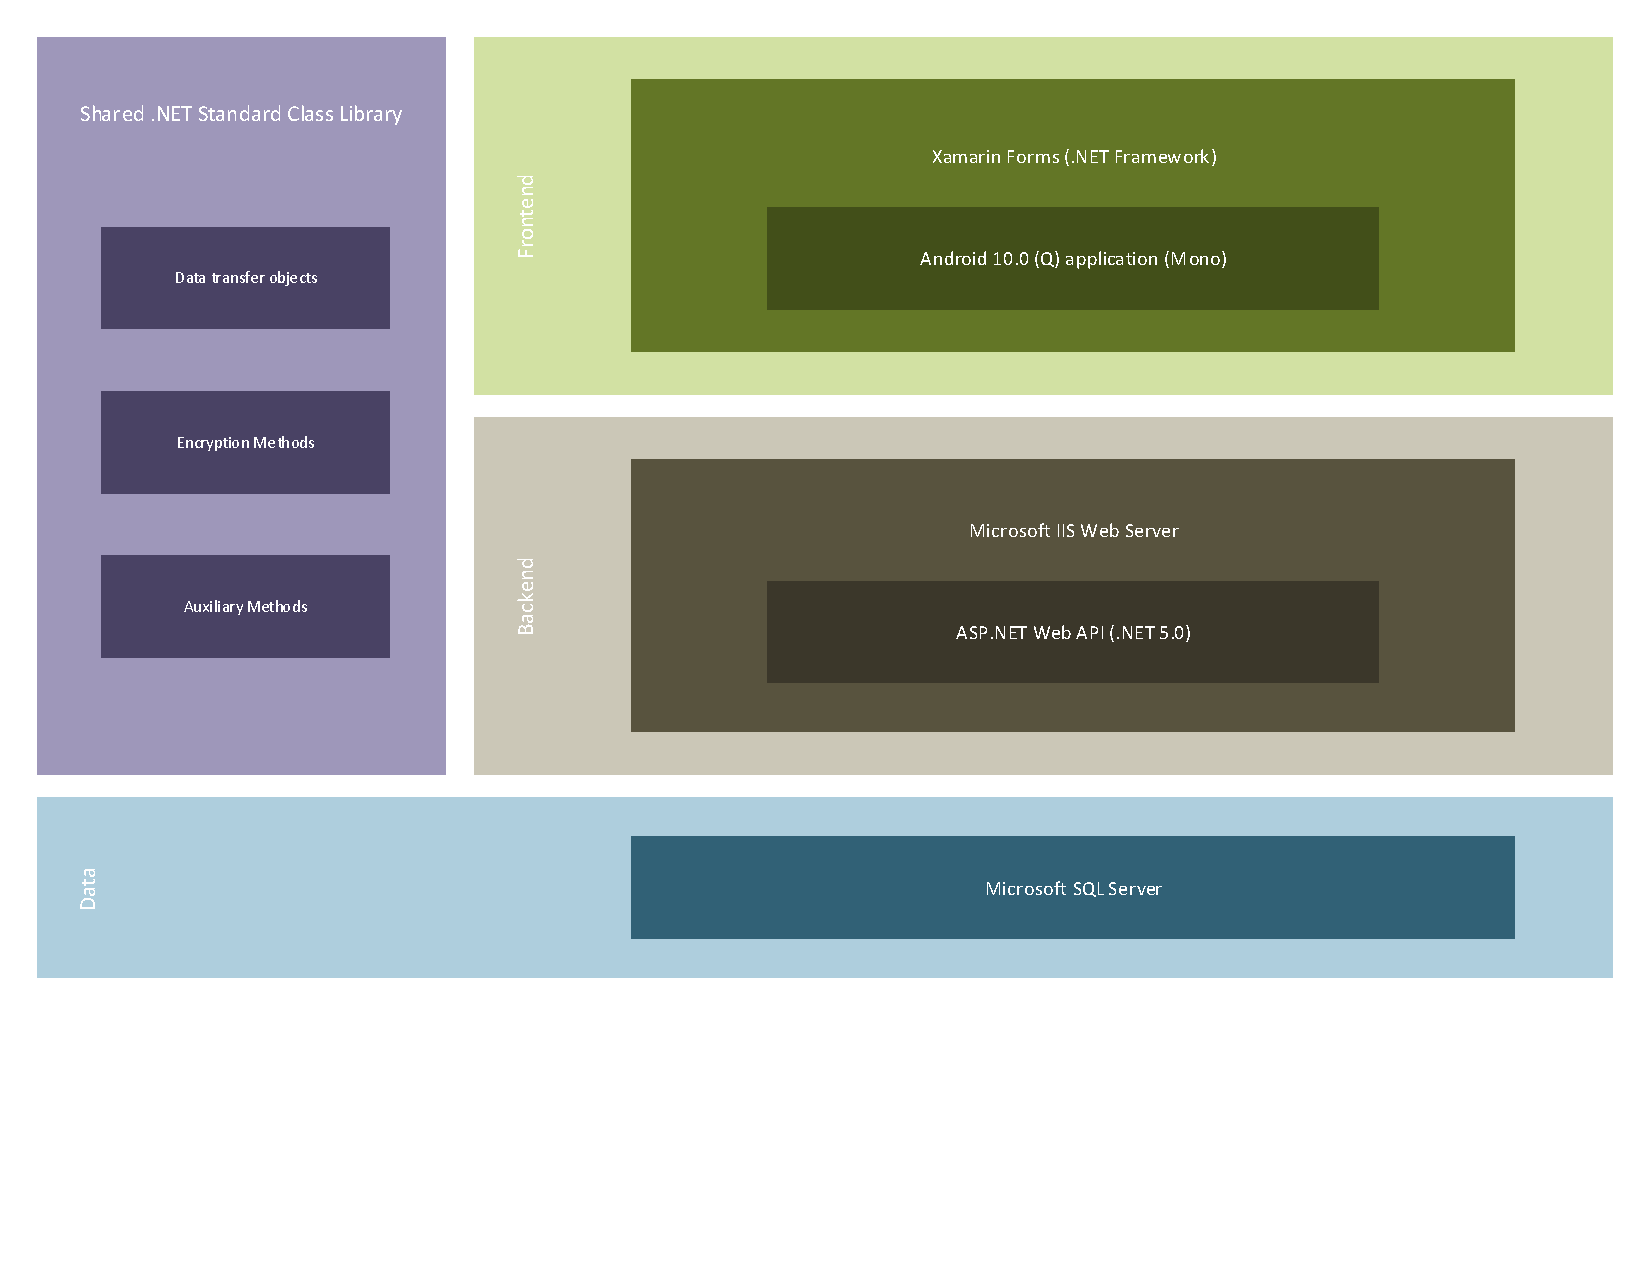
\includegraphics[scale=0.57]{general-architecture}
	\caption{General architecture}
\end{figure}

Along with the low cost of change, the independence of the layers allows for efficient future expansion of 
the application by means of multiple frontend platforms (ex. web applications, desktop applications), cloud storage/services and additional
Web API's that can easily be integrated into the existing application.
This, combined with the high compatibility of the .NET 5.0, provides a high level of scalability and maintainability for the application.

The application and presentation layers share a common class library that contains communication-related models and auxiliary methods.
This library allows both layers to benefit from the cross-platform nature of .NET 5.0, speeding up the process of development and
ensuring there are no discrepancies betweeen the layers in terms of encryption and communication.

\subsection{Application layer / Backend}

The architecture of the application layer has a similar design approach to the general architecture.
Consisting of 4 layers, the backend follows the single-responsibility principle in it's core.
Because of it's vertical structure, each layer is dependent on one single layer that is directly below it, providing a high level
of maintainability.

\begin{figure}[H]
	\centering
	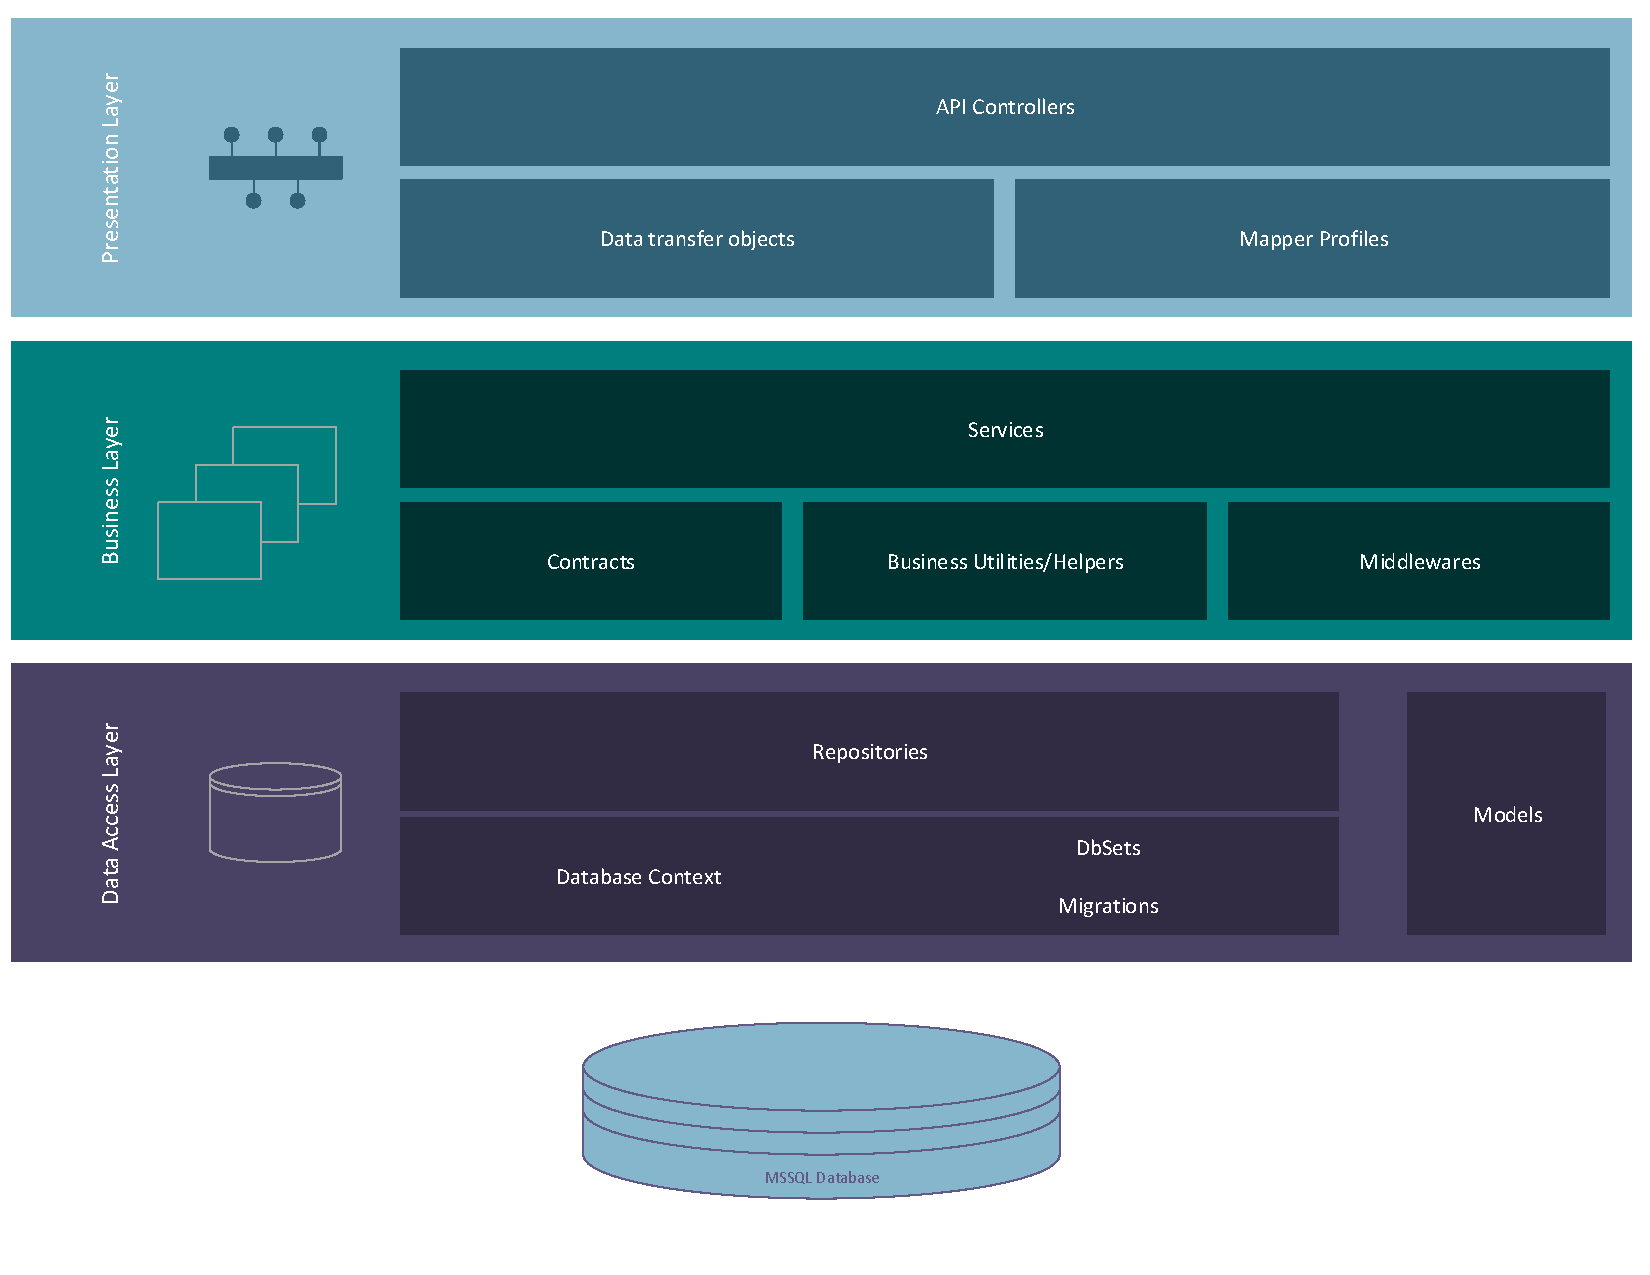
\includegraphics[scale=0.57]{backend-architecture}
	\caption{Backend architecture}
\end{figure}

Due to this abstract layout, each layer can independently be replaced or updated. 
This aspect enables the utilization of external and/or third-party services and components without damaging the integrity of the application.

The API structure of the presentation layer allows for a wide variety of applications or even services in which the backend can be used: desktop applications,
WPF, web servers and more. This characteristic has major role in preserving the flexibility of the application layer.

Another component being responsible for the independece and reusability of the backend is the Data Access Layer. 
The role of this layer is to provide the data requested by the Business Layer. 
By reason of abstraction, this layer is independent of the technology of the data source. 
This enables the utilization of a wide range of data sources, including relational (SQL) and non-relational (NoSQL) databases, cloud services and/or APIs.

\subsubsection{Entity relations in the application layer}


\begin{figure}[H]
	\centering
	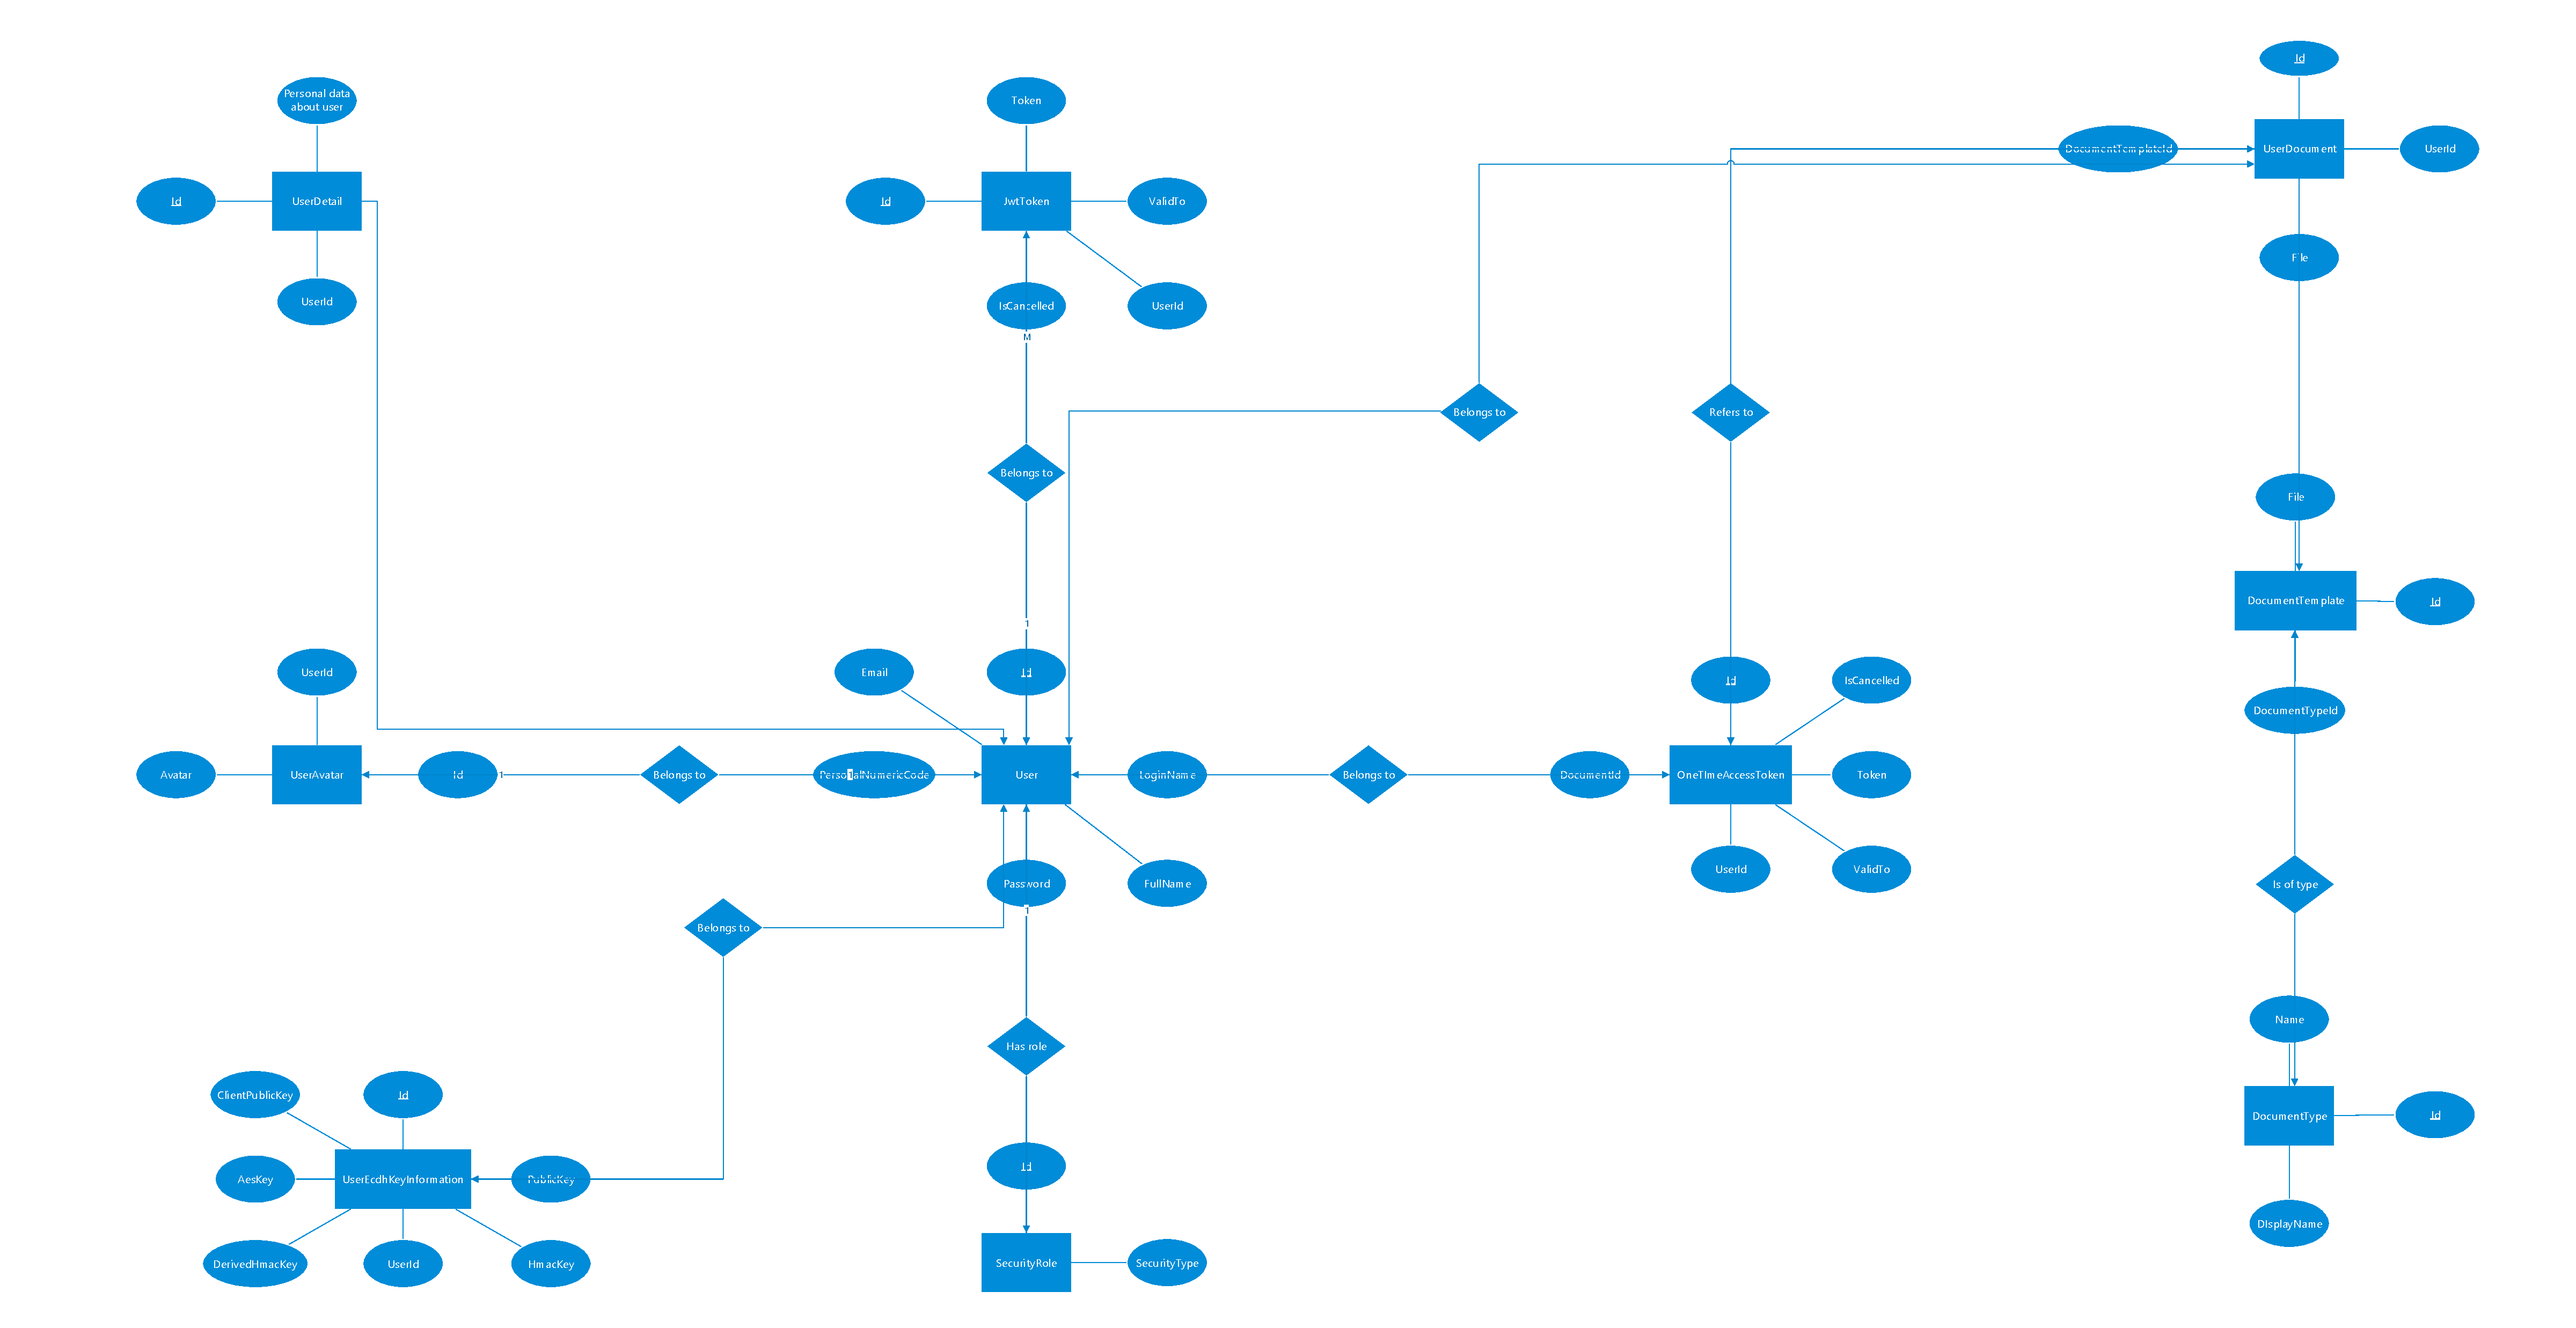
\includegraphics[scale=0.29]{entity-relationship-diagram}
	\caption{ER diagram}
\end{figure}

\subsection{Presentation layer / Frontend}

The frontend of the application consists of three major layers that separate the user interface from the business logic and the data sources.
This separation allows for easy horizontal expansion and quick feature development.

The Presentation or UI Layer contains the visuals of the application which are separated into independent pages, however it is also responsible for receiving
user events and connecting them with the underlying services.
Each page contains it's own event listeners and separate View Model that is responsible for making use of the Business Layer,
which has a similar structure and role to the backend's Business Layer: data processing and calculations.

The main components of the Data Layer are Data Stores.
These stores are functionally similar to the repositories found in the Backend of the application, although here the data is retrieved using the endpoints
of the backend.

\begin{figure}[H]
	\centering
	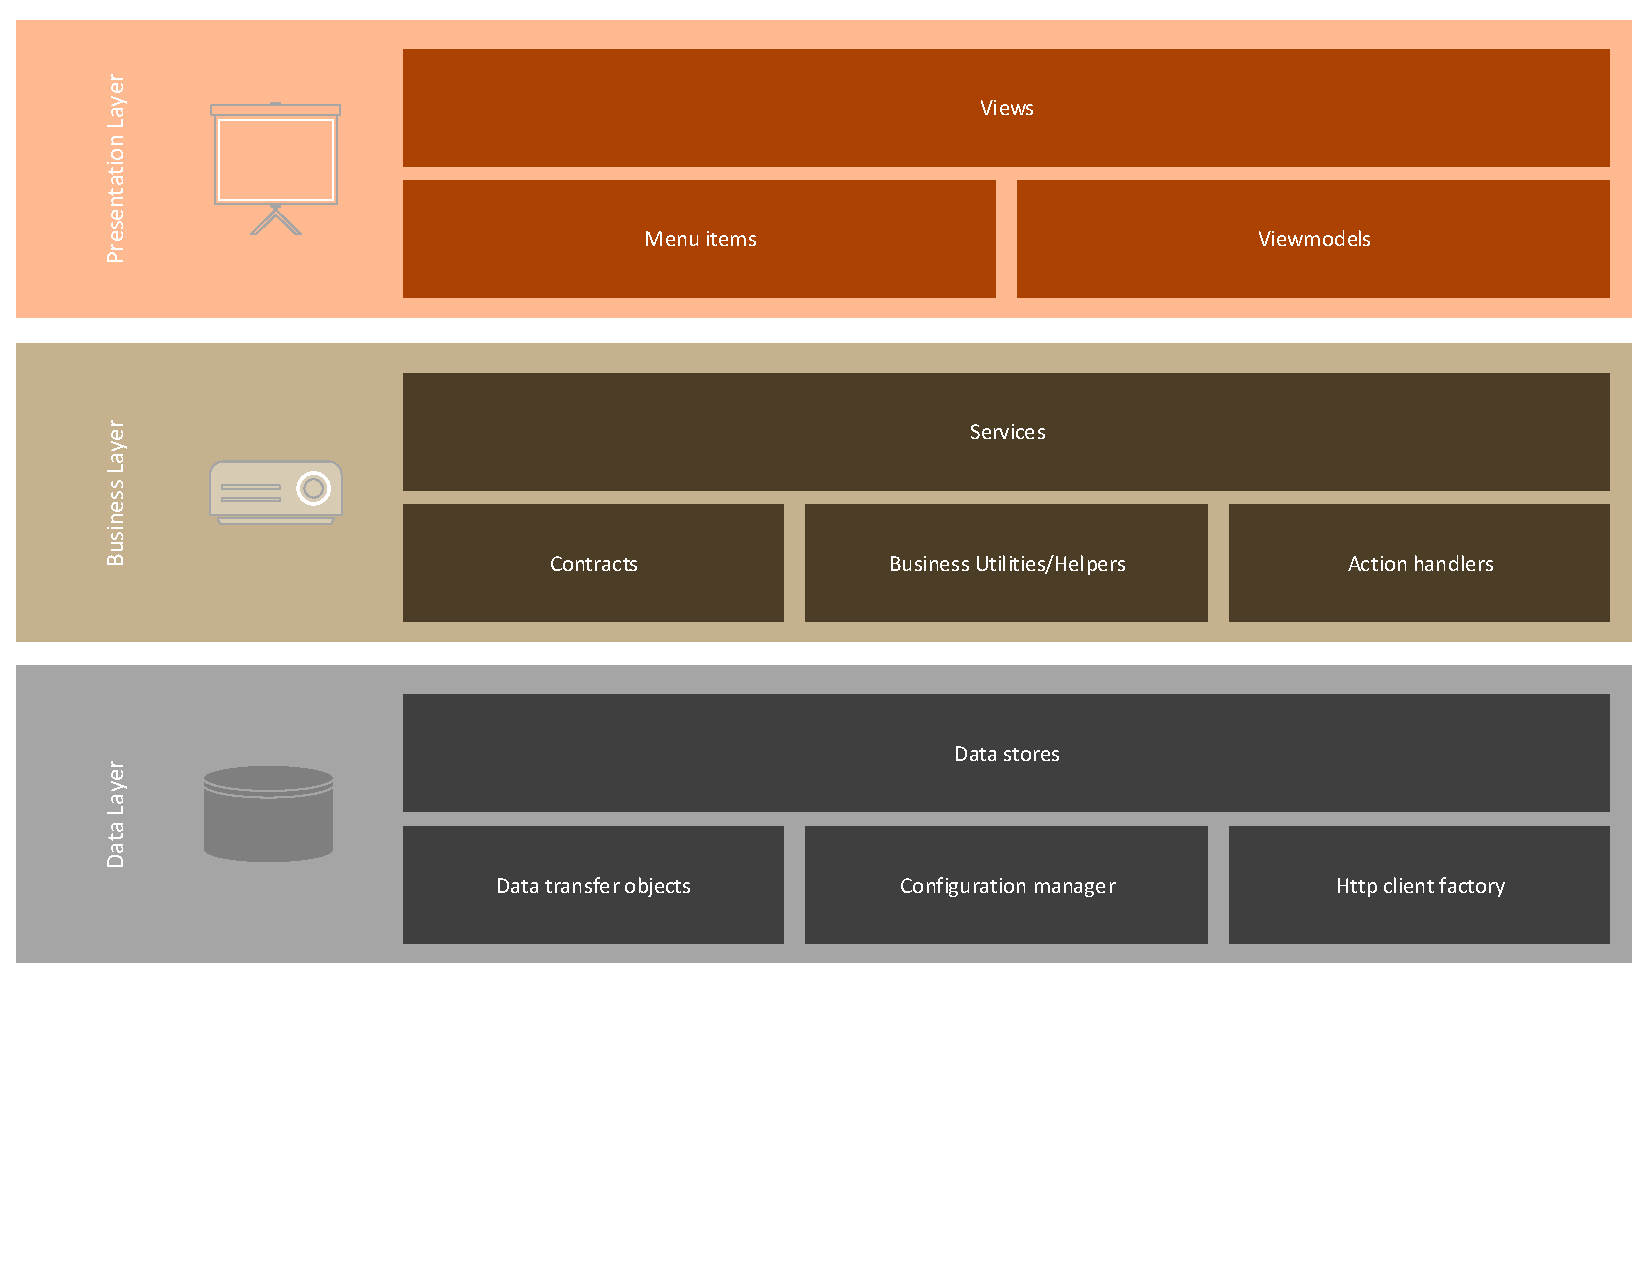
\includegraphics[scale=0.57]{frontend-architecture}
	\caption{Frontend architecture}
\end{figure}


%%%%%%%%%%%%%%%%%%%%%%%%%%%%%%%%%%%%%%%%%%%%%%%%%%%%%%%%%%%%%%%%%%%%%%%
\section{Technologies}

E-me makes great use of the cross-platform nature of .NET, meaning both the frontend and the backend of the application are implemented using the same
programming language: C\# 9.
The flexibility that is provided by the language and the wide variety of frameworks that make use of it allows for a cleaner codebase and a simpler
project structure when compared to a multilingual application design.

\subsection{Backend}

In terms of frameworks, the backend relies on .NET 5.0. Being the next major release of .NET Core following 3.1, this open-source cross-platform
software framework unifies a wide variety of frameworks .NET has to offer, including Windows Forms, ASP.NET Core, Azure and more.
This unification made the framework a perfect candidate for the backend of an application like E-me, since it can be used on a wide variety of
platforms and ensures long-term support.

E-me uses Internet Information Services (Microsoft IIS), which is an extensible web server software, as it's backend server.
It allows the application to communicate through HTTPS and provides it's separate development-time SSL certificate in order to secure the transport
layer. With the \emph{Development-time IIS support} feature, the web server allows \emph{hot reloading}, which speeds up the development and debugging
processes.

The main constituent of the backend itself is the ASP.NET Core web framework.
Using it's built-in IoC, this framework allows for a high level of abstraction in order to build well-structured enterprise level applications
using dependency injection.
This framework is responsible for registering and configuring any other dependencies that may appear in the application backend.

Alongside with ASP.NET Core, one of the main components of the backend is the Entity Framework Core, which is the base of the 
\emph{Data Access Layer}.
In terms of building and maintaining the data access layer, E-me uses the code-first approach through \emph{EF Migrations}.
This approach provides flexibility in case of a potential database change and/or creation, but more importantly it allows 
the entire structure of the entities to be managed based on the models and datasets present in the code.

Although the frameworks used by the layers of the application differ, these can have a shared codebase in the form
of a \emph{.NET Standard class library}, which can be used by both the backend and the frontend.

\begin{itemize}
	\item Backend
	\begin{itemize}
		\item .NET 5
		\item Entity Framework Core 5
		\begin{itemize}
			\item Code-first
			\item Microsoft SQL Server
			\item additional Data Encryption layer
		\end{itemize}
		\item NSwag
		\item Serilog
		\item AutoMapper
		\item Newtonsoft Json
		\item Windows CNG (Cryptographic Next Generation) API
	\end{itemize}
	\item Frontend
	\begin{itemize}
		\item Xamarin Forms
		\item Telerik UI for Xamarin
		\item Telerik Document Processing Core
		\item Syncfusion Xamarin PDF viewer
		\item GoogleVision API - BarcodeScanner XF implementation
	\end{itemize}
\end{itemize}

\section{Implementation}


\section{Security}
Here I describe the Diffie-Hellman key exchange and the used encryption techniques in more detail, 3-4 pages.

\begin{itemize}
	\item data-layer security
	\begin{itemize}
		\item using built-in EF Data Encryption with AES256
	\end{itemize}
	\item transport-layer security (TLS)
	\begin{itemize}
		\item https
		\item JWT auth and auth verification
		\item protected and unprotected endpoints
	\end{itemize}
	\item End-To-End encryption
	\begin{itemize}
		\item Elliptic Curve Diffie-Hellman key derivation - open-source implementation
		\item encryption of documents
		\item hash-based message authentication (HMAC)
	\end{itemize}
\end{itemize}